\documentclass[a4paper, 12pt]{article}

% packages
\usepackage{amssymb}
\usepackage[fleqn]{mathtools}
\usepackage{tikz}
\usepackage{enumerate}
\usepackage{bussproofs}
\usepackage{xcolor}
\usepackage[margin=1.3cm]{geometry}
\usepackage{logicproof}
\usepackage{diagbox}
\usepackage{listings}
\usepackage{graphicx}
\usepackage{lstautogobble}
\usepackage{hyperref}
\usepackage{multirow}
\usepackage{tipa}
\usepackage{pgfplots}
\usepackage{adjustbox}

% tikz libraries
\usetikzlibrary{
    decorations.pathreplacing,
    arrows,
    shapes,
    shapes.gates.logic.US,
    circuits.logic.US,
    calc,
    automata,
    positioning,
    intersections
}

\pgfplotsset{compat=1.16}

\pgfmathdeclarefunction{gauss}{2}{%
  \pgfmathparse{1/(#2*sqrt(2*pi))*exp(-((x-#1)^2)/(2*#2^2))}%
}

\allowdisplaybreaks % allow environments to break
\setlength\parindent{0pt} % no indent

% shorthand for verbatim
% this clashes with logicproof, so maybe fix this at some point?
\catcode`~=\active
\def~#1~{\texttt{#1}}

% code listing
\lstdefinestyle{main}{
    numberstyle=\tiny,
    breaklines=true,
    showspaces=false,
    showstringspaces=false,
    tabsize=2,
    numbers=left,
    basicstyle=\ttfamily,
    columns=fixed,
    fontadjust=true,
    basewidth=0.5em,
    autogobble,
    xleftmargin=3.0ex,
    mathescape=true
}
\newcommand{\dollar}{\mbox{\textdollar}} %
\lstset{style=main}

% augmented matrix
\makeatletter
\renewcommand*\env@matrix[1][*\c@MaxMatrixCols c]{%
\hskip -\arraycolsep
\let\@ifnextchar\new@ifnextchar
\array{#1}}
\makeatother

% ceiling / floor
\DeclarePairedDelimiter{\ceil}{\lceil}{\rceil}
\DeclarePairedDelimiter{\floor}{\lfloor}{\rfloor}

% custom commands
\newcommand{\indefint}[2]{\int #1 \, \mathrm{d}#2}
\newcommand{\defint}[4]{\int_{#1}^{#2} #3 \, \mathrm{d}#4}
\newcommand{\pdif}[2]{\frac{\partial #1}{\partial #2}}
\newcommand{\dif}[2]{\frac{\mathrm{d}#1}{\mathrm{d}#2}}
\newcommand{\limit}[2]{\raisebox{0.5ex}{\scalebox{0.8}{$\displaystyle{\lim_{#1 \to #2}}$}}}
\newcommand{\limitsup}[2]{\raisebox{0.5ex}{\scalebox{0.8}{$\displaystyle{\limsup_{#1 \to #2}}$}}}
\newcommand{\summation}[2]{\sum\limits_{#1}^{#2}}
\newcommand{\product}[2]{\prod\limits_{#1}^{#2}}
\newcommand{\intbracket}[3]{\left[#3\right]_{#1}^{#2}}
\newcommand{\laplace}{\mathcal{L}}
\newcommand{\fourier}{\mathcal{F}}
\newcommand{\mat}[1]{\boldsymbol{#1}}
\renewcommand{\vec}[1]{\boldsymbol{#1}}
\newcommand{\rowt}[1]{\begin{bmatrix}
    #1
\end{bmatrix}^\top}
\DeclareMathOperator*{\argmax}{argmax}
\DeclareMathOperator*{\argmin}{argmin}

\newcommand{\lto}[0]{\leadsto\ }

\newcommand{\ulsmash}[1]{\underline{\smash{#1}}}

\newcommand{\powerset}[0]{\wp}
\renewcommand{\emptyset}[0]{\varnothing}

\makeatletter
\newsavebox{\@brx}
\newcommand{\llangle}[1][]{\savebox{\@brx}{\(\m@th{#1\langle}\)}%
  \mathopen{\copy\@brx\kern-0.5\wd\@brx\usebox{\@brx}}}
\newcommand{\rrangle}[1][]{\savebox{\@brx}{\(\m@th{#1\rangle}\)}%
  \mathclose{\copy\@brx\kern-0.5\wd\@brx\usebox{\@brx}}}
\makeatother
\newcommand{\lla}{\llangle}
\newcommand{\rra}{\rrangle}
\newcommand{\la}{\langle}
\newcommand{\ra}{\rangle}
\newcommand{\crnr}[1]{\text{\textopencorner} #1 \text{\textcorner}}
\newcommand{\bnfsep}[0]{\ |\ }
\newcommand{\concsep}[0]{\ ||\ }

\newcommand{\axiom}[1]{\AxiomC{#1}}
\newcommand{\unary}[1]{\UnaryInfC{#1}}
\newcommand{\binary}[1]{\BinaryInfC{#1}}
\newcommand{\trinary}[1]{\TrinaryInfC{#1}}
\newcommand{\quaternary}[1]{\QuaternaryInfC{#1}}
\newcommand{\quinary}[1]{\QuinaryInfC{#1}}
\newcommand{\dproof}[0]{\DisplayProof}
\newcommand{\llabel}[1]{\LeftLabel{\scriptsize #1}}
\newcommand{\rlabel}[1]{\RightLabel{\scriptsize #1}}

\newcommand{\ttbs}{\char`\\}
\newcommand{\lrbt}[0]{\ \bullet\ }

% colours
\newcommand{\violet}[1]{\textcolor{violet}{#1}}
\newcommand{\blue}[1]{\textcolor{blue}{#1}}
\newcommand{\red}[1]{\textcolor{red}{#1}}
\newcommand{\teal}[1]{\textcolor{teal}{#1}}

% reasoning proofs
\usepackage{ltablex}
\usepackage{environ}
\keepXColumns
\NewEnviron{reasoning}{
    \begin{tabularx}{\textwidth}{rlX}
        \BODY
    \end{tabularx}
}
\newcommand{\proofline}[3]{$(#1)$ & $#2$ & \hfill #3 \smallskip \\}
\newcommand{\proofarbitrary}[1]{& take arbitrary $#1$ \smallskip \\}
\newcommand{\prooftext}[1]{\multicolumn{3}{l}{#1} \smallskip \\}
\newcommand{\proofmath}[3]{$#1$ & = $#2$ & \hfill #3 \smallskip \\}
\newcommand{\prooftherefore}[1]{& $\therefore #1$ \smallskip \\}
\newcommand{\proofbc}[0]{\prooftext{\textbf{Base Case}}}
\newcommand{\proofis}[0]{\prooftext{\textbf{Inductive Step}}}

% ER diagrams
\newcommand{\nattribute}[4]{
    \node[draw, state, inner sep=0cm, minimum size=0.2cm, label=#3:{#4}] (#1) at (#2) {};
}
\newcommand{\mattribute}[4]{
    \node[draw, state, accepting, inner sep=0cm, minimum size=0.2cm, label=#3:{#4}] (#1) at (#2) {};
}
\newcommand{\dattribute}[4]{
    \node[draw, state, dashed, inner sep=0cm, minimum size=0.2cm, label=#3:{#4}] (#1) at (#2) {};
}
\newcommand{\entity}[3]{
    \node[] (#1-c) at (#2) {#3};
    \node[inner sep=0cm] (#1-l) at ($(#1-c) + (-1, 0)$) {};
    \node[inner sep=0cm] (#1-r) at ($(#1-c) + (1, 0)$) {};
    \node[inner sep=0cm] (#1-u) at ($(#1-c) + (0, 0.5)$) {};
    \node[inner sep=0cm] (#1-d) at ($(#1-c) + (0, -0.5)$) {};
    \draw
    ($(#1-c) + (-1, 0.5)$) -- ($(#1-c) + (1, 0.5)$) -- ($(#1-c) + (1, -0.5)$) -- ($(#1-c) + (-1, -0.5)$) -- cycle;
}
\newcommand{\relationship}[3]{
    \node[] (#1-c) at (#2) {#3};
    \node[inner sep=0cm] (#1-l) at ($(#1-c) + (-1, 0)$) {};
    \node[inner sep=0cm] (#1-r) at ($(#1-c) + (1, 0)$) {};
    \node[inner sep=0cm] (#1-u) at ($(#1-c) + (0, 1)$) {};
    \node[inner sep=0cm] (#1-d) at ($(#1-c) + (0, -1)$) {};
    \draw
    ($(#1-c) + (-1, 0)$) -- ($(#1-c) + (0, 1)$) -- ($(#1-c) + (1, 0)$) -- ($(#1-c) + (0, -1)$) -- cycle;
}

% AVL Trees
\newcommand{\avltri}[4]{
    \draw ($(#1)$) -- ($(#1) + #4*(0.5, -1)$) -- ($(#1) + #4*(-0.5, -1)$) -- cycle;
    \node at ($(#1) + #4*(0, -1) + (0, 0.5)$) {#3};
    \node at ($(#1) + #4*(0, -1) + (0, -0.5)$) {#2};
}

% RB Trees
\tikzset{rbtr/.style={inner sep=2pt, circle, draw=black, fill=red}}
\tikzset{rbtb/.style={inner sep=2pt, circle, draw=black, fill=black}}

% Samples
\tikzset{spos/.style={inner sep=2pt, circle, draw=black, fill=blue!20}}
\tikzset{sneg/.style={inner sep=2pt, circle, draw=black, fill=red!20}}

% Joins
\newcommand\ljoin{\stackrel{\mathclap{\normalfont\mbox{\tiny L}}}{\bowtie}}
\newcommand\rjoin{\stackrel{\mathclap{\normalfont\mbox{\tiny R}}}{\bowtie}}
\newcommand\ojoin{\stackrel{\mathclap{\normalfont\mbox{\tiny O}}}{\bowtie}}

\setcounter{MaxMatrixCols}{100}

% actual document
\begin{document}
    {\sc Computing $4^\text{th}$ Year Notes} \hfill ~https://github.com/lin-e/imperial-revision~
    \rule{\textwidth}{0.1pt}
    \section*{Scalable Systems and Data \hfill (70022)}
        \subsection*{1.1 - Database Storage Layer}
            This lecture covers the DBMS layers, storage hierarchy as well as the role disks takes in the DBMS.
            The DBMS layers are as follows, with the query going into the first layer, and storage being the final layer.
            Note that the last two layers (buffer management and disk space management are typically done by the OS).
            \begin{enumerate}[1.]
                \itemsep0em
                \item \textbf{query optimization and execution} \hfill tries to reorganise the query to execute efficiently
                \item \textbf{relational operators}
                \item \textbf{file and access methods} \hfill understand which files need to be accessed and indexes we can use
                \item \textbf{buffer management} \hfill handles reading disk pages and buffering in main memory for fast access
                \item \textbf{disk space management}
            \end{enumerate}
            An example of this could be a search engine, which is much simpler than a general DBMS - albeit having similar layers;
            \begin{enumerate}[1.]
                \itemsep0em
                \item search string modifier
                \item ranking engine
                \item query execution
                \item buffer management
                \item disk space management
            \end{enumerate}
            This is simpler than a DBMS as it can simply use the OS for the bottom two layers, there is typically no concurrency (nor any need for transactions, being mostly read-only), and typically has hard-wired queries.
            The ranking engine and query execution is a simple DBMS.
            \subsubsection*{DBMS versus Using OS}
                An important question is why we don't simply use the OS.
                The layers of abstractions can be useful, but we have a lot of knowledge on how to access the data.
                In addition, the OS can often get in the way of the DBMS - it has some idea on what to query and what files to touch, and knows more about the OS regarding future access, which can be exploited.
                A DBMS needs to do things its own way, for example specialised pre-fetching with the knowledge of future access.
                Additionally, if we control the buffer management, we can also control the replacement policy, likely with something better than the OS.
                With more control over the thread / process scheduling, the DBMS can achieve a more optimal execution of the workflow as the DB locks aren't going to conflict with the OS locks (high contention).
                There's also control over flushing data to the disk, including writing log file (important for recovery), and shouldn't be left to the OS.
            \subsubsection*{Disks and Files}
                Today, disks are still the go-to storage medium for large amounts of files, and have become fairly affordable (not as affordable as tape for archival storage, but much cheaper than other media, such as SSD or main memory).
                Unlike other media, disks have mechanical parts leading to differences access patterns or behaviour - the time to access a piece of data is affected by \textbf{where} the data is on the disk.
                A lot of databases today are still on disks, as it's cheap with a reasonable access time - typically the data is read from the disk onto main memory (buffered), and changes are written back to the disk from the buffer.
                \medskip

                High-end databases are in the petabyte range, therefore using main memory would be extremely expensive.
                In addition to that, main memory is volatile - meaning the data is lost if power goes out.
                However, main-memory databases do exist for smaller sized, performance optimised systems, in which volatility is tolerable.
                \medskip

                Flash storage isn't commonly used in DBMS as main storage (due to the cost), but can also be used as an accelerator or enabler, in the form of a specialised cache, etc.
                \medskip

                The storage hierarchy is as follows.
                Note that flash storage can either be used to the side of magnetic disk (for a specific portion of the files), or as a buffer on top (before main memory).
                \textit{Jim Gray} has an analogy for how far away the data is (registers being knowledge in your head, etc), illustrating the scale of access time.
                \begin{center}
                    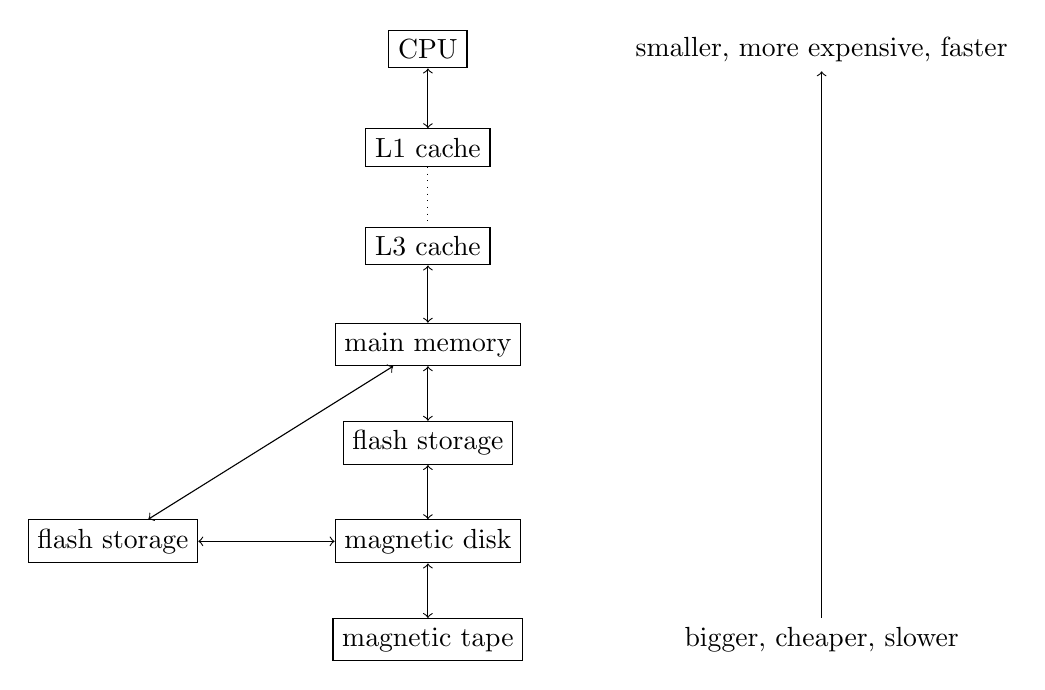
\begin{tikzpicture}[y=1.25cm]
                        \node[draw] (cpu) at (0, 0) {CPU};
                        \node[draw] (l1) at (0, -1) {L1 cache};
                        \node[draw] (l3) at (0, -2) {L3 cache};
                        \node[draw] (mm) at (0, -3) {main memory};
                        \node[draw] (fs1) at (0, -4) {flash storage};
                        \node[draw] (md) at (0, -5) {magnetic disk};
                        \node[draw] (fs2) at (-4, -5) {flash storage};
                        \node[draw] (mt) at (0, -6) {magnetic tape};

                        \draw
                        (cpu) edge[<->] (l1)
                        (l1) edge[dotted] (l3)
                        (l3) edge[<->] (mm)
                        (mm) edge[<->] (fs1)
                        (mm) edge[<->] (fs2)
                        (fs1) edge[<->] (md)
                        (fs2) edge[<->] (md)
                        (md) edge[<->] (mt);

                        \node (x) at (5, -6) {bigger, cheaper, slower};
                        \node (y) at (5, 0) {smaller, more expensive, faster};

                        \draw (x) edge[->] (y);
                    \end{tikzpicture}
                \end{center}
                Disks are still the main secondary storage device of choice, with the main advantage over tapes being the ability to perform random access, rather than purely sequential.
                Data is stored in units in \textbf{disk blocks} or \textbf{pages} (may be used interchangeably), typically in the order of kilobytes and occasionally megabytes.
                Unlike RAM, the time to retrieve / write a disk page varies depending on the location, with a tremendous impact on time to retrieve, hence relative placement of pages on a disk has a major impact on performance.
                The lecture then goes over the anatomy of a disk;
                \begin{itemize}
                    \itemsep0em
                    \item spindle and platters spin between 5,000 - 15,000 RPM (with physical limitations)
                    \item arm assembly has multiple disk head, one for each platter - the tracks under the heads form a cylinder
                    \item only one head reads or writes at once
                \end{itemize}
                The time to access a disk block has three elements;
                \begin{itemize}
                    \itemsep0em
                    \item \textbf{seek time} \hfill time to move the arm to the correct position (in and out, towards the spindle)
                    \item \textbf{rotational delay} \hfill arm assembly in a fixed position, block needs to be rotated under head
                    \item \textbf{transfer time} \hfill actual time to read data from disk into main memory
                \end{itemize}
                The time for a smaller number of cylinders traversed is dominated by the seek time (head positioning).
                In modern disks, short seeks are dominated by the \textbf{settle time}, which gets larger with increased disk track density.
                \medskip

                Generally, the seek time and rotational delay dominates, with the former being in the range of 1 to 20ms, and the latter being in the range of 0 to 10ms.
                On the other hand, the transfer rate is less than 1 millisecond for a 4KB page.
                As such, the key to lower I/O cost is to reduce the delays caused by seek and rotation.
                Additionally, in shared disks, most of the time is spent waiting for access to the arm.
                \medskip

                The concept of the next block is as follows;
                \begin{itemize}
                    \itemsep0em
                    \item blocks on the same track, followed by
                    \item blocks on the same cylinder
                    \item blocks on adjacent cylinder
                \end{itemize}
                We can't control where we write on the disk - that's controlled by the device driver.
                Typically, if data is written together, it will also be read together.
                Defragmentation is disk optimization, as data can be spread out all over a disk for a given file, leading to slower read times - this is done by putting all the pieces of a file closer together.
                \medskip

                Note that an adjacent block doesn't necessarily mean physically adjacent.
                Data can be physically spread out over a disk but in a certain pattern that can lead to near sequential access.
                The adjacent blocks can be the blocks under the disk head after rotating during settle time.
                \medskip

                In general, memory access is much faster than disk I/O (roughly $1,000 \times$), and sequential I/O is faster than random (roughly $10 \times$).
                \medskip

                The lowest layer of DBMS manages the space on the disk and higher levels can call this layer to allocate / de-allocate a page, or read / write a page.
            \subsubsection*{Summary}
                In general, the key for storing data on a disk is to store data together if it's queried together.
                Random access should be avoided, preferably use sequential access.
                Data structures should be aligned for page size - for example, if a data structure were to have a few bytes in the next page, an additional page would have to be retrieved, despite mostly being irrelevant.
\end{document}